\thispagestyle{lichsutoanhocnone}
\pagestyle{lichsutoanhoc}
\graphicspath{{../lichsutoanhoc/pic/}}
\everymath{\color{lichsutoanhoc}}
\blfootnote{$^1$\color{lichsutoanhoc}Cộng tác viên Viện Toán học.}
\begingroup
\AddToShipoutPicture*{\put(0,616){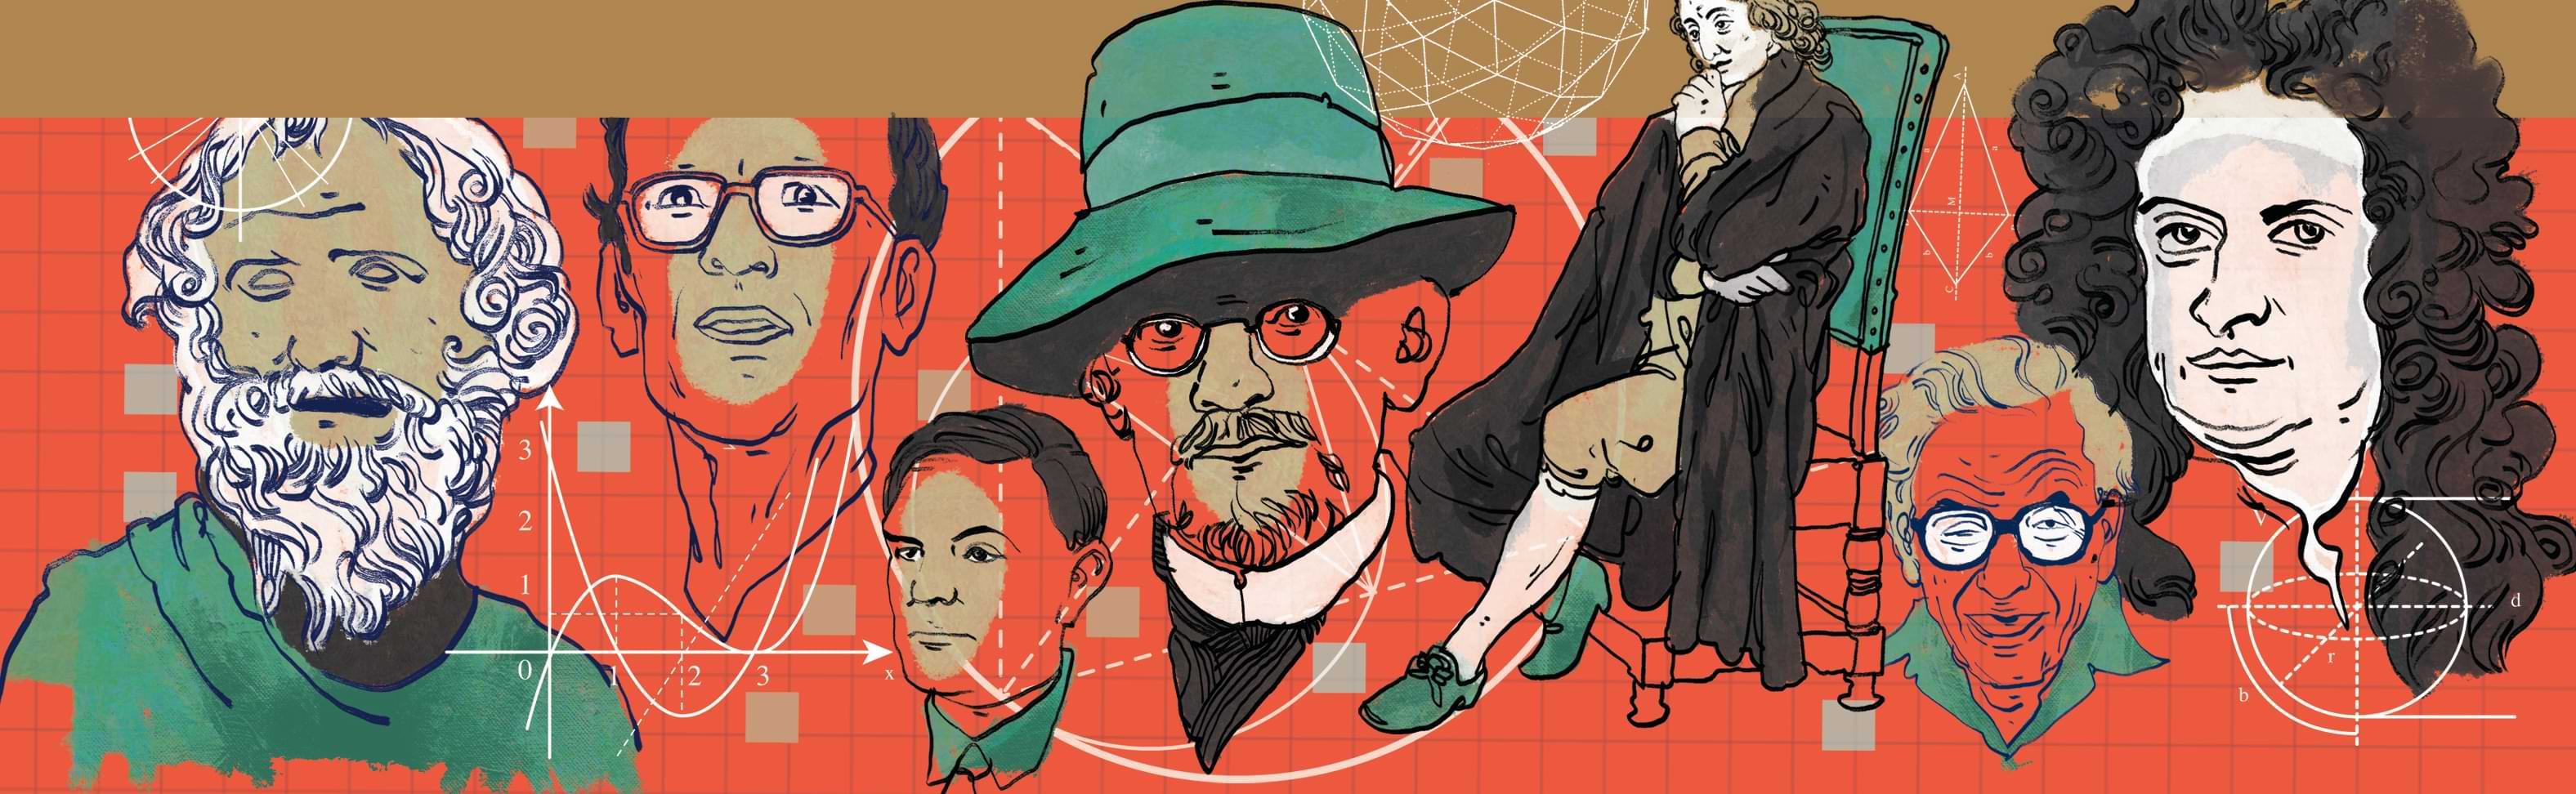
\includegraphics[width=19.3cm]{../bannerlichsu}}}
\AddToShipoutPicture*{\put(100,515){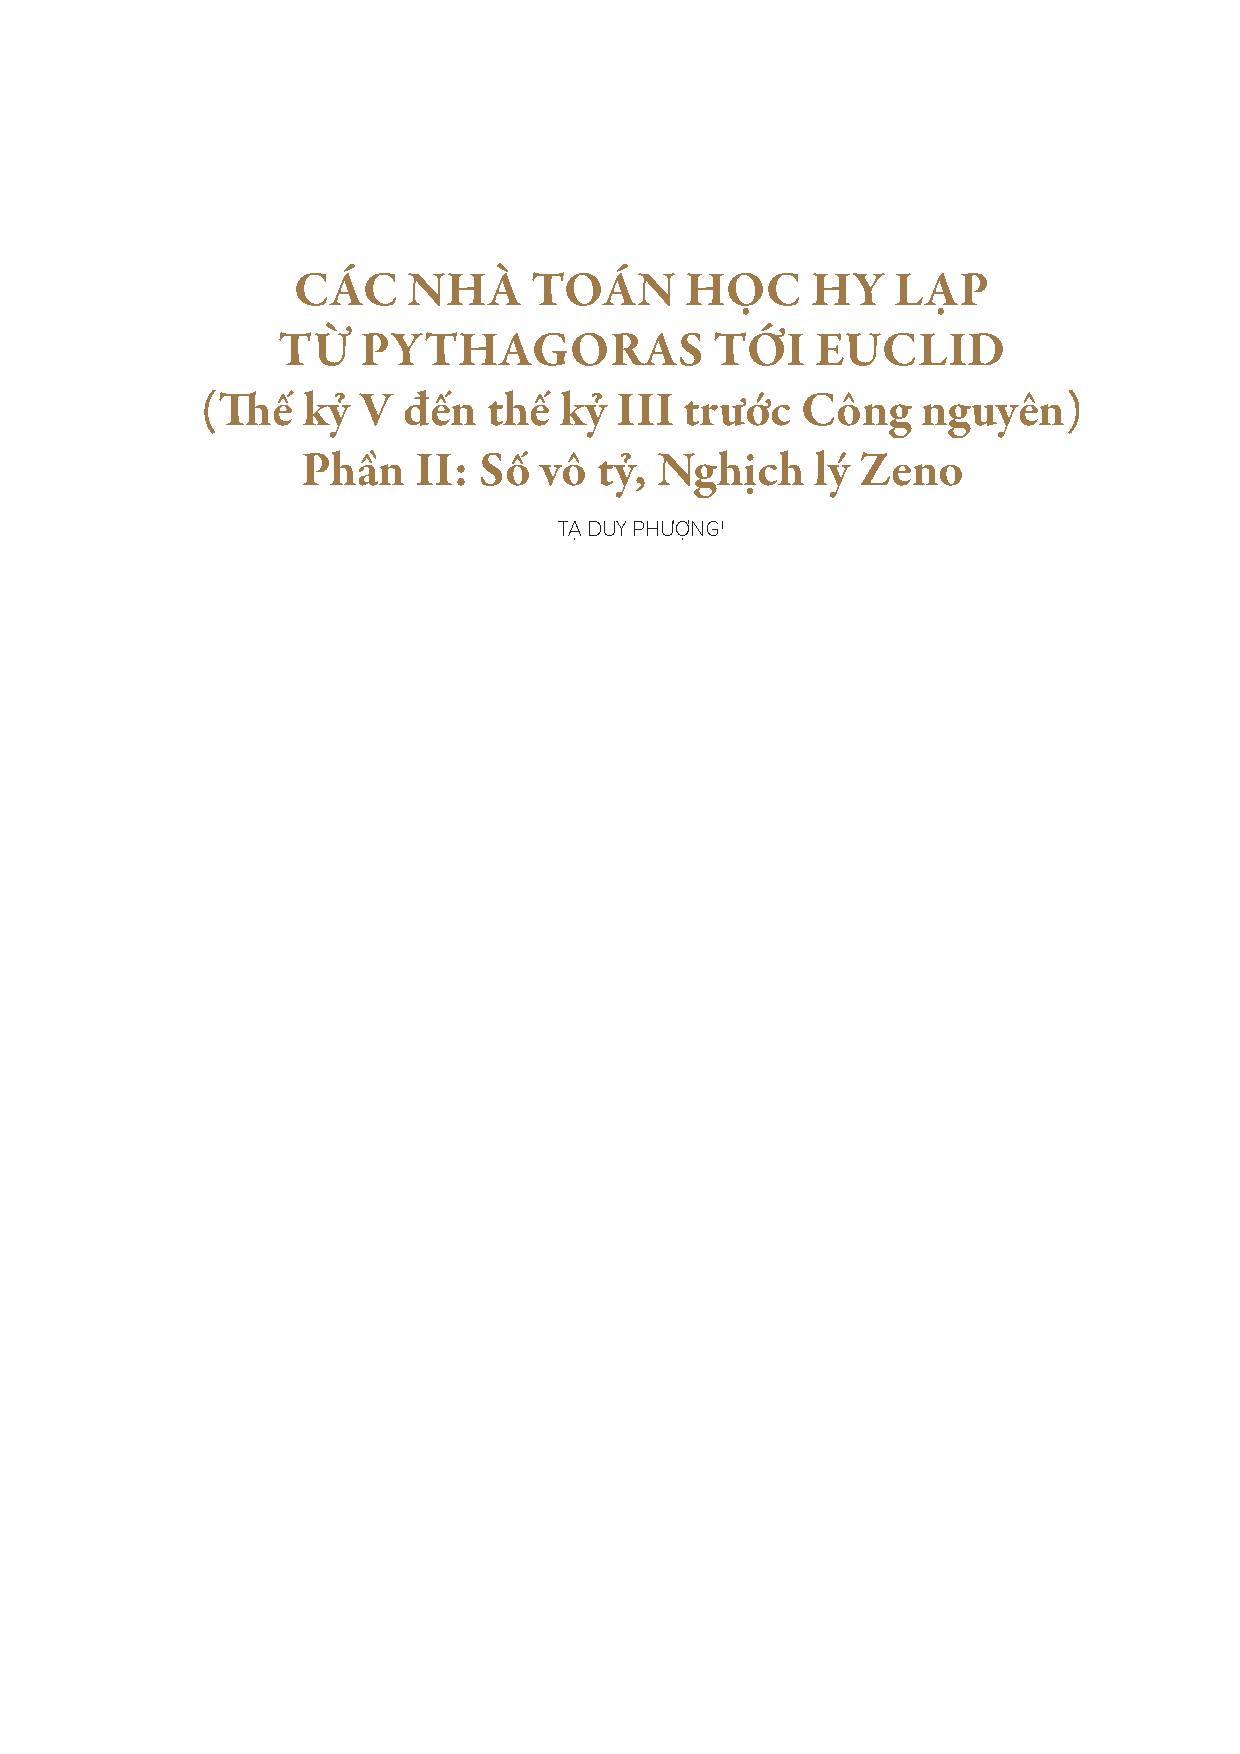
\includegraphics[scale=1]{../tieude.pdf}}}
\centering
\endgroup

\vspace*{200pt}

\begin{multicols}{2}
	\textbf{Lời dẫn:} Tiếp thu những thành tựu thiên văn học và toán học của người Babylon và người Ai Cập, người Hy Lạp đã đẩy toán học lên thành một ngành khoa học độc lập, với các triết lí và phương pháp riêng. Toán học Hy Lạp đã phát triển rực rỡ trong $1000$ năm, từ năm $600$ trước Công nguyên đến năm $400$ Công nguyên. Người đặt nền móng cho toán học Hy Lạp là nhà toán học, thiên văn học và triết học Thales. Ông là người đứng đầu và là nhà toán học duy nhất trong \textit{Bảy nhà thông thái Hy Lạp} (Seven Sages of Greece).
		\begin{figure}[H]
		\centering
		\vspace*{-5pt}
		\captionsetup{labelformat= empty, justification=centering}
		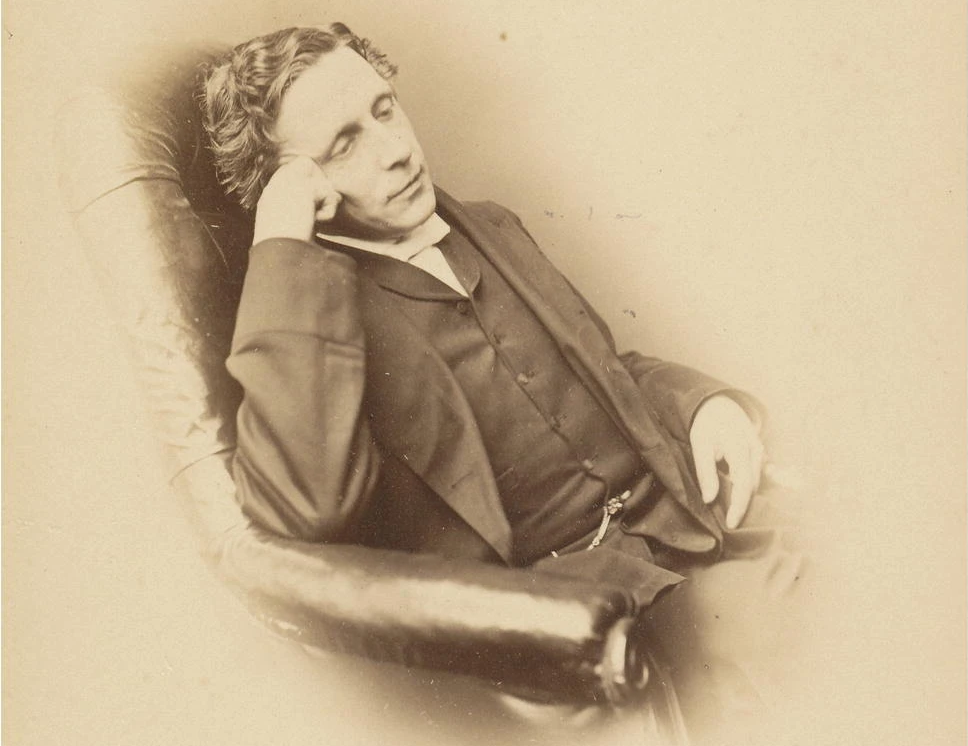
\includegraphics[width=1\linewidth]{1}
		\caption{\small\textit{\color{lichsutoanhoc}Hình $1$: Bảy nhà thông thái Hy Lạp.}}
		\vspace*{-10pt}
	\end{figure}
	\textbf{Tiểu sử}
	\vskip 0.1cm
	Thales (khoảng $625 - 547$ trước Công nguyên) là người gốc Phoenicia, sinh ra ở Miletus, một thành phố của Ionia, khi đó thuộc Hy Lạp, hiện nay thuộc Thổ Nhĩ Kỳ. 
		\begin{figure}[H]
		\centering
		\vspace*{-5pt}
		\captionsetup{labelformat= empty, justification=centering}
		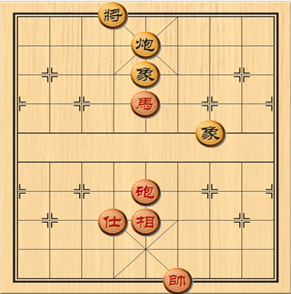
\includegraphics[width=1\linewidth]{2}
		\caption{\small\textit{\color{lichsutoanhoc}Hình $2$: Bản đồ đế chế Hy Lạp.}}
		\vspace*{-10pt}
	\end{figure}
	Hồi trẻ ông theo nghề buôn. Ông được coi là người sắc sảo và thông minh trong nghề. Và trong các chuyến đi của mình, Ông đã học toán từ người Ai Cập và thiên văn từ người Babylon.
	\vskip 0.1cm
	\textbf{Thales -- nhà toán học} 
	\vskip 0.1cm
	Toán học Ai Cập về cơ bản là tập hợp các công cụ và kĩ thuật được định hình để giải các bài toán thực tế. Dựa trên những nguyên liệu thô nhưng phong phú này của người Ai Cập, người Hy Lạp đã tái tạo lại thành các nguyên tắc chung, qua đó làm cho kiến thức toán học trở nên tổng quát và dễ hiểu hơn, đồng thời khám phá ra nhiều điều mới. Thí dụ, “diện tích cánh đồng ngũ cốc hình tam giác” cụ thể đã được trừu tượng và tổng quát thành “diện tích hình tam giác”.
		\begin{figure}[H]
		\centering
		\vspace*{-5pt}
		\captionsetup{labelformat= empty, justification=centering}
		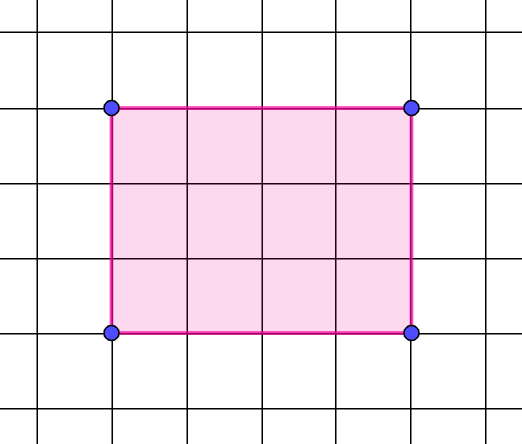
\includegraphics[width=0.65\linewidth]{3}
		\caption{\small\textit{\color{lichsutoanhoc}Hình $3$:  Thales (Khoảng $625 - 547$ trước Công nguyên).}}
		\vspace*{-10pt}
	\end{figure}
	\textbf{Phương pháp suy diễn}
	\vskip 0.1cm
	Thales được công nhận là người đầu tiên chứng minh các khẳng định toán học nhờ logic dựa trên lập luận suy diễn thay cho thực nghiệm và trực giác. Nhà triết học Proclus (khoảng $412 - 485$) trong cuốn \textit{Commentary on the First Book of Euclid’s Elements}  (Chú giải cuốn sách \textit{Cơ sở}  của Euclid) đã viết: \textit{“Thales là người đầu tiên  đưa hình học Ai Cập vào Hy Lạp. Ông còn tự mình tìm ra nhiều mệnh đề [...], trong một số trường hợp, các phương pháp của ông là tổng quát, trong những trường hợp khác mang tính thực nghiệm.”}
	Thales đã đóng góp cho hình học những định lý sau đây, được đưa vào \textit{Cơ sở} của Euclid:
	\vskip 0.1cm
	$1)$  Hai đường thẳng cắt nhau tạo nên các góc đối đỉnh bằng nhau.\footnote[2]{Mệnh đề $I.15$, $[1]$ trang $131$; $[6]$ trang $41$.}
	\vskip 0.1cm
	$2)$  Đường tròn bị chia làm hai phần bằng nhau bởi đường kính của nó.\footnote[3]{$[1]$, trang $131$}
	\vskip 0.1cm 
	$3)$ Góc nội tiếp chắn nửa đường tròn là góc vuông.\footnote[4]{$[1]$, trang $131$}
	\vskip 0.1cm 
	$4)$ Hai góc ở đáy của tam giác cân bằng nhau.\footnote[5]{Mệnh đề $I.5$, $[1]$, trang $131$ hoặc $[6]$, trang $27$}
	\vskip 0.1cm
	$5)$ Các cạnh của hai tam giác đồng dạng tương ứng tỉ lệ.\footnote[6]{Mệnh đề $VI.4$, $[1]$ trang $131$; $[6]$, trang $294$} 
	\vskip 0.1cm
	$6)$ Hai tam giác bằng nhau nếu chúng có một cạnh và hai góc kề với nó tương ứng bằng nhau. \footnote[7]{Mệnh đề $I.26$, $[1]$ trang $131$; $[6]$, trang $56$).
	\vskip 0.1cm 
	Định lí đảo của Định lí $3)$ cũng đúng. Định lí $3)$ có nhiều ứng dụng. Dưới đây là hai Thí dụ.
	\vskip 0.1cm
	\textbf{Thí dụ} $\pmb{1.}$ \textit{Xác định tâm hình  tròn nhờ sử dụng một thước thợ (thước vuông) và một thước thẳng.}
	\vskip 0.1cm
	\textbf{Lời giải:}
	\textbf{Bước $\pmb{1}$:} Đặt đỉnh của thước vuông trên đường tròn. Hai cạnh của thước vuông cắt đường tròn tại hai điểm. 
	\vskip 0.1cm
	\textbf{Bước $\pmb{2}$:} Lấy thước kẻ nối hai điểm vừa nhận được. Đây chính là một đường kính của đường tròn. 
	\vskip 0.1cm
	\textbf{Bước $\pmb{3}$:} Đặt đỉnh thước thợ vào một điểm khác và làm lại Bước $1$ và Bước $2$, được đường kính thứ hai. Giao của hai đường kính chính là tâm đường tròn (Hình $4$). 
	\begin{figure}[H]
		\centering
		\vspace*{-5pt}
		\captionsetup{labelformat= empty, justification=centering}
		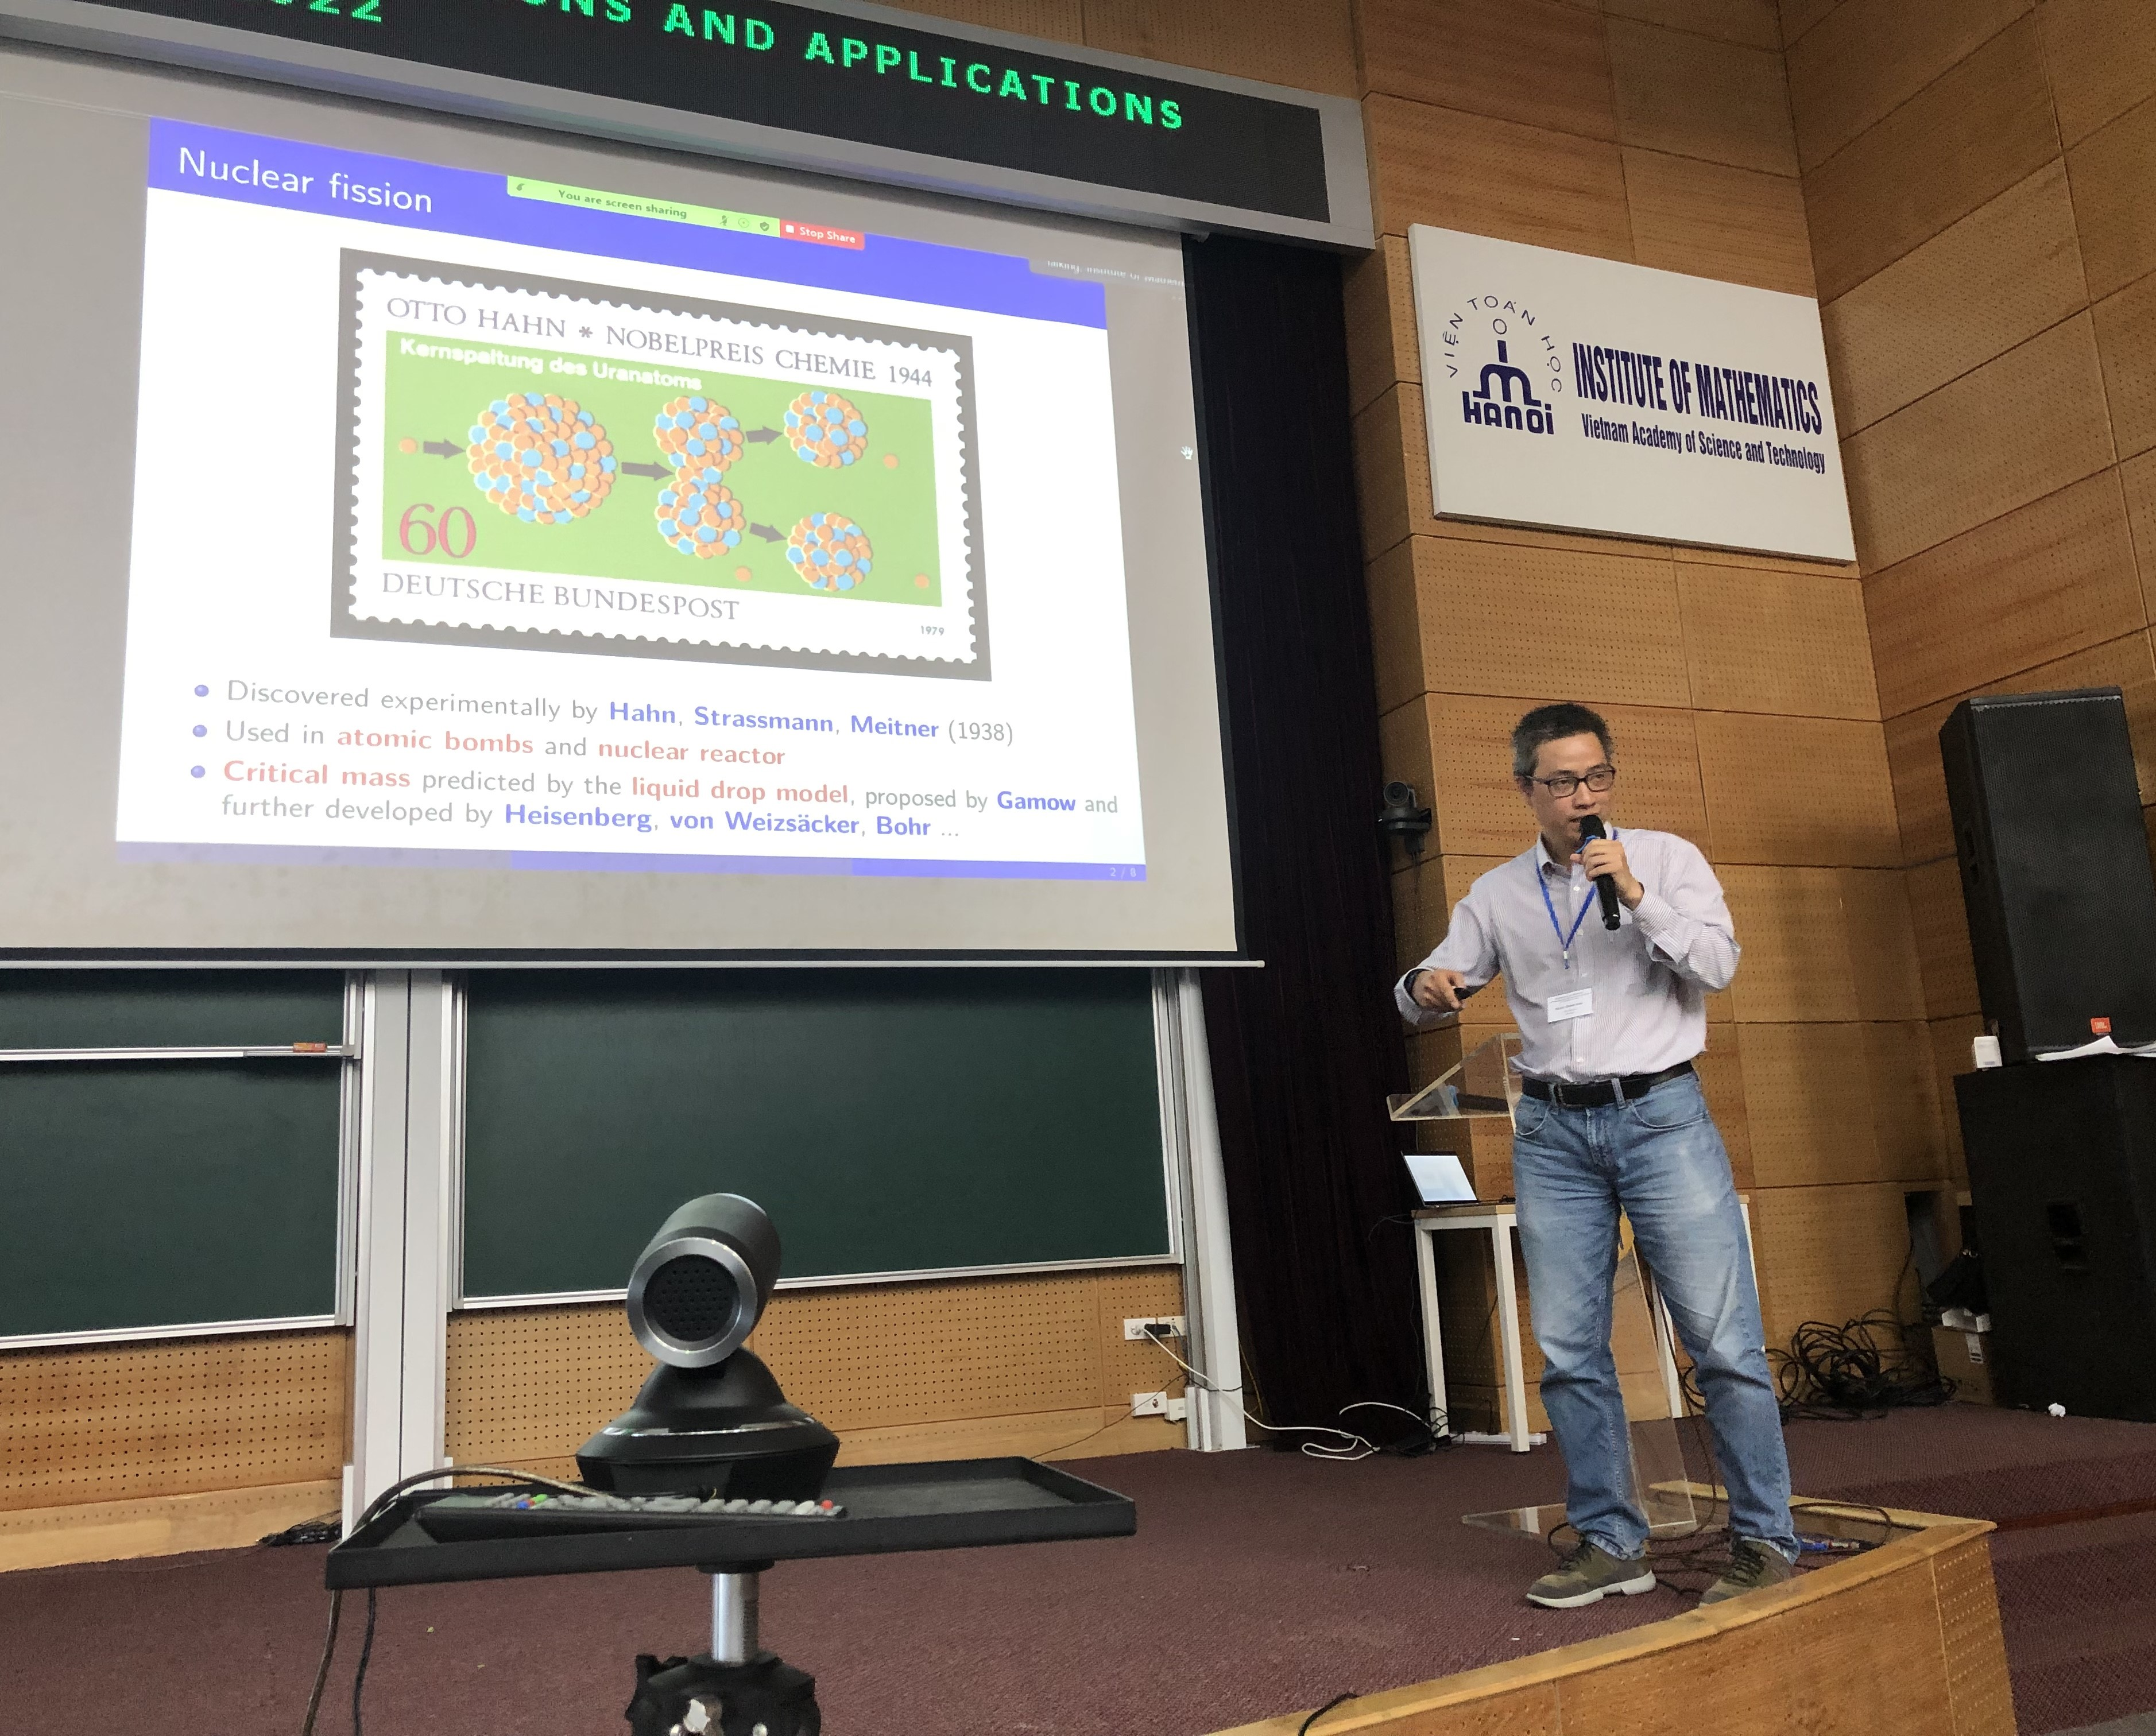
\includegraphics[width=1\linewidth]{4}
		\caption{\small\textit{\color{lichsutoanhoc}Hình $4$: Xác định tâm hình tròn.}}
		\vspace*{-10pt}
	\end{figure}
	\textbf{Thí dụ $\pmb{2}$.} Từ một điểm $P$ cho trước kẻ tiếp tuyến tới đường tròn tâm  $O$ cho trước.
	\vskip 0.1cm
	\textbf{Lời giải:} Đường tròn đường kính $OP$  cắt đường tròn tâm $O$  tại hai điểm $T$   và $T'$.  Khi ấy $PT$  và $PT'$  là hai tiếp tuyến cần tìm (Hình $5$).
	\begin{figure}[H]
		\centering
		\vspace*{-5pt}
		\captionsetup{labelformat= empty, justification=centering}
		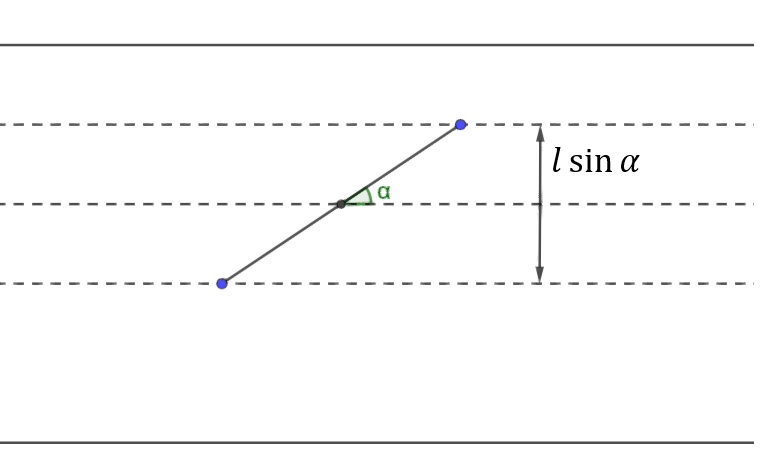
\includegraphics[width=1\linewidth]{5}
		\caption{\small\textit{\color{lichsutoanhoc}Hình $5$: Kẻ tiếp tuyến tới đường tròn.}}
		\vspace*{-10pt}
	\end{figure}
	Đóng góp quan trọng nhất của Thales trong toán học là ông đã đưa ra một phương pháp chứng minh thống nhất: phương pháp suy diễn logic, tức là từ giả thiết, nhờ một dãy các suy luận logic dựa trên những điều đã được công nhận (các định nghĩa và tiên đề) và các điều đã được chứng minh (các định lí và mệnh đề), dẫn đến điều cần chứng minh. Điều này đã giúp người Hy Lạp đưa toán học, đặc biệt là hình học lên một tầm cao mới, thành một hệ thống chặt chẽ và thống nhất. Do đó, nhiều học giả coi Thales là \textit{nhà hình học đầu tiên} và định lí \textit{Một đường thẳng song song với cạnh đáy của tam giác tạo ra một tam giác mới có các cạnh tỉ lệ với các cạnh của tam giác cũ} (Hình $6$) được mang tên \textit{Định lí Thales}.
	\vskip 0.1cm
	\textbf{Giả thiết:} $BC \parallel B'C'$.
	\vskip 0.1cm    
	Kết luận: $\frac{AB}{AB'} = \frac{AC}{AC'} = \frac{BC}{B'C'}$.
	\vskip 0.1cm
	Tỉ lệ trên vẫn được bảo toàn khi ta tịnh tiến hoặc quay tam giác $ABC$ (Hình $6$, bên phải). Tức là, \textit{nếu hai tam giác có các góc bằng nhau, thì các cạnh của chúng tương ứng tỉ lệ}. Các tam giác như vậy được gọi là \textit{tam giác đồng dạng}.
	\begin{figure}[H]
		\centering
		\vspace*{-5pt}
		\captionsetup{labelformat= empty, justification=centering}
		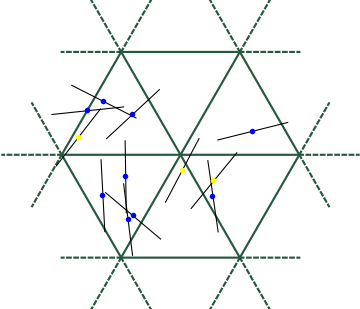
\includegraphics[width=1\linewidth]{6}
		\caption{\small\textit{\color{lichsutoanhoc}Hình $6$: Định lí Thales.}}
		\vspace*{-10pt}
	\end{figure}
	Christopher Clavius (1538-1612) và  François Viète (1540-1603) đã phát triển khái niệm tam giác đồng dạng của Thales thành khái niệm hình đồng dạng:. 
	
	Hình 7: Hình đồng dạng phối cảnh.
	Hai hình   và   được gọi là đồng dạng (phối cảnh) với nhau theo tâm     tỉ số   nếu với mỗi điểm    có thể tìm được điểm   (và ngược lại, với mỗi điểm    có thể tìm được điểm  ) sao cho  
	Từ Định lí Thales suy ra, nếu các hình   và   và   đồng dạng phối cảnh với nhau tâm   tỉ số   thì với mỗi cặp điểm, thí dụ,  , có thể tìm được các cặp điểm   và  sao cho  
	và  
	Tương tự,    (Hình 7).
	
	Ứng dụng tam giác đồng dạng 
	đĐĐo chiều cao của Đại Kim tự tháp 
	Có hai giai thoại nói về chuyện Thales đã đo chiều cao của Đại Kim tự tháp. Giai thoại thứ nhất kể rằng Thales đã cắm một cây gậy dưới bóng nắng mặt trời. Khi bóng của cây gậy dài bằng chiều cao của nó, ông đo bóng của kim tự tháp và suy ra chiều cao của nó. Giai thoại thứ hai do nhà thơ, nhà viết sử Hy Lạp Plutarch  (46 - -120) viết trong tác phẩm Convivium (Bữa tiệc): “Mặc dù ông ta [Vua Hy Lạp] ngưỡng mộ anh [Thales] về rất nhiều điều, nhưng ông đặc biệt ngưỡng mộ anh bởi cái cách anh đo Đại Kim tự tháp mà không cần dụng cụ nào.”
	
	Hình 8: Đại Kim tự tháp Giza (Cheops).
	Cả hai giai thoại đều dựa trên một mệnh đề hình học (của Thales): Hai tam giác có các góc tương ứng  bằng nhau (nói cách khác, hai tam giác đồng dạng) thì các cạnh của chúng tương ứng tỉ lệ. Tức là:    
	,
	trong đó    và    là chiều cao và chiều dài bóng (tính từ tâm) của kim tự tháp, còn    và    là chiều cao và chiều dài bóng của cây gậy (xem Hhình bên 9dưới). 
	Thales đã biết cạnh đáy của Đại Kim tự tháp   foot nên khoảng cách từ tâm kim tự tháp ra đến cửa bằng    foot. Cây gậy dài 6 foot, bóng của cây gậy bằng 9 foot. Khoảng cách từ cửa đến bóng của đỉnh Kim tự tháp bằng 342 foot. Suy ra  foot. Vậy chiều cao kim tự tháp là 
	foot.
	Hình 9: Đo chiều cao Đại Kim tự thápThales đã biết cạnh đáy của Đại Kim tự tháp bằng.  foot (1 foot = 0,3048 m) nên khoảng cách từ tâm kim tự tháp ra đến cửa bằng  foot. Cây gậy dài 6 foot, bóng của cây gậy bằng 9 foot. Khoảng cách từ cửa đến bóng của đỉnh Kim tự tháp bằng 342 foot. Suy ra foot. Vậy chiều cao kim tự tháp là foot.
	
	
	
	Đo khoảng cách tới tàu biển 
	Một ứng dụng khác của tam giác đồng dạng là đo khoảng cách từ bờ tới tàu đang ở ngoài biển. 
	
	Hình 10: Tính khoảng cách đếên tàu.
	Giả sử    là vị trí của tàu,  tháp có đáy là điểm  chiều cao tháp là   chiều cao của người quan sát đứng trên đỉnh tháp có chiều cao là là    điểm   (mắt người), vị trí   của tàu và điểm  thẳng hàng,     là các khoảng cách có thể đo được và điểm   (mắt người), vị trí   của tàu và điểm   thẳng hàng. Từ hai tam giác đồng dạng    và     ta có  :  Suy ra khoảng cách
	từ bờ tới tàu bằng   
	Một cách khác để đo khoảng cách từ điểm   trên bờ biển tới con tàu   là dựng một đoạn   trên bờ biển vuông góc với  Mắt người đặt ở điểm  trên đường vuông góc với   tại   Đường thẳng   cắt  tại   Như vậy,   thẳng hàng.Từ hai tam giác vuông đồng dạng   và   ta có   
	Vì      đo được nên  (Hình 11)
	
	
	Hình 11: Tính khoảng cách đến tàu, đồn địch
	Bài toán trên còn được áp dụng trong quân sự, khi cần đo khoảng cách từ trận địa pháo đến điểm  là đồn địch (điểm không tới được).
	Thales - nhà thiên văn 
	Đương thời, Thales nổi tiếng là một nhà thiên văn hơn là một nhà toán học. Ông đã tính được một năm có 365 ngày. Ông giải thích hiện tượng nhật thực diễn ra là do mặt trăng che khuất mặt trời. Một truyền thuyết hay được nhắc lại là người Hy Lạp rất ngạc nhiên khi Thales đã tiên đoán đúng nhật thực vào ngày 28 tháng 5 năm 585 trước Công nguyên. Nhà sử học Hy Lạp Herodotus (khoảng 484 - 425 trước Công nguyên) đã ghi lại rằng sự kiện này diễn ra trong một trận chiến giữa người Lydia và người Media. Và khi ngày chuyển sang đêm (do nhật thực), cuộc chiến chấm dứt. Các vị vua đã kinh hoàng đến mức họ đã kí kết một nền hòa bình lâu dài.
	
	Một số giai thoại vui về Thales 
	Mọi người đều nhất trí đánh giá Thales là một người sắc sảo và thông minh không chỉ trong khoa học, mà cả trong chính trị và thương mại. Nhiều giai thoại, một số là nghiêm túc, một số là huyền ảo, kể về sự thông minh của ông. Dưới đây là một vài giai thoại về Thales.   
	
	Chuyện buôn ô liu 
	Theo Aristotle (nhà triết học và bác học Hy Lạp, 384 - 322 trước Công nguyên), có một lần, sau nhiều năm liền cây ô liu không ra quả. B, bằng kiến thức thiên văn của mình, Thales đã dự đoán mùa tới sẽ bội thu. Ông liền mua tất cả các máy ép ô liu xung quanh Miletus, quê ôÔng. Khi mùa thu hoạch đến, do có độc quyền quản lí máy ép, ông đã đưa ra giá thuê chúng theo ý ông, và do đó đã thu được một khoản tiền lớn. Một số người cho rằng, Thales muốn chứng minh quan điểm của mình là, các triết gia, nếu họ muốn, rất dễ trở nên giàu có.
	Chuyện buôn muối 
	Thales có một đàn la chở muối đi bán. Ông tình cờ quan sát thấy một số con la dìm mình xuống nước khi qua suối, do đó muối bị tan ra và la được chở nhẹ hơn. Lần sau, ông cho những con la đó chở những tấm bọt biển. Khi la dìm mình xuống nước, bọt biển thấm nước làm la phải chở nặng hơn. Từ đó trở đi, la thông minh không dám dìm mình xuống nước nữa.
	
	Chuyện mải ngắm sao vấp ngã 
	
	Theo Plato (nhà triết học Hy Lạp, khoảng 424 - 348 trước Công nguyên), một lần vào buổi đêm, Thales ra ngoài đi dạo, do mải ngắm sao, ông đã ngã xuống một con mương. Một bà già, sau khi đã giúp Thales lên được bờ, đã nói với ông: “Làm sao ông có thể nói được gì đang diễn ra trên bầu trời, trong khi ông không nhìn thấy gì dưới chân?” Câu chuyện này thường được nhắc tới trong thời cổ đại để minh họa bản chất thiếu thực tế của các học giả. Và có lẽ nó vẫn phần nào còn đúng trong thời đại ngày nay.
	
	Thay lời kết 
	Các bạn học sinh có thể băn khoăn ngạc nhiên khi thấy bài viết chỉ liệt kê 6 mệnh đề đơn giản trong hình học được gán tên Thales,, vì bạn cũng có thể tự phát hiện và chứng minh chúng, và các mệnh đề này cũng đã có trong các sách giáo khoa hình học.. Nhưng bạn hãy trở về 2600 năm trước, khi toán học mới chỉ là một mớ các công cụ nhằm giải quyết các bài toán thực tế cụ thể, các bạn sẽ thấy sự vĩ đại của Thales. Vấn đề không chỉ ở kĩ thuật chứng minh một định lí hay một khẳng định toán học cụ thể, mà quan trọng là ý tưởng và phương pháp chung giải các lớp bài toán tổng quát. 
	Mặc dù các công trình của ông không còn được lưu giữ, các kết quả của Ôông chủ yếu do người đời sau viết lại, Thales vẫn giữ một vị trí rất cao trong toán học. Ông là người tiên phong đưa vào trong toán phép chứng minh bằng diễn dịch (từ một số giả thiết ban đầu và những điều đã biết suy ra một dãy các khẳng định đúng, và cuối cùng suy ra điều cần chứng minh), góp phần phát triển hình học thành một ngành khoa học độc lập. Ngoài ra, ông cũng là một nhà thiên văn và nhà triết học duy vật nổi tiếng cho đến tận ngày nay.
	Người Trung Quốc cũng đã biết đến ứng dụng của tam giác đồng dạng từ thế kỉ III (xem [7]). Người Việt Nam đầu tiên biết đến đồng dạng là Lương Thế Vinh (1441 - 1496). Ông đã có bài toán đo chiều cao của cây theo bóng của nó (xem  [8]). Kĩ thuật đo chiều cao, đo độ sâu và đo khoảng cách nhờ tam giác đồng dạng, tương tự bài toán tính khoảng cách từ bờ đến con tàu ngoài khơi của Thales, nhưng tiện dụng hơn trong thực tế nhờ sử dụng hai cột biểu, cũng đã được Ý Trai Nguyễn Hữu Thận (1757 - 1831) và một số tác giả Việt Nam khác đề cập (xem  [8]). 
	Mặc dù các công trình của Ôông không còn được lưu giữ, Thales vẫn giữ một vị trí rất cao trong toán học, vì Ôông là người tiên phong đưa vào trong toán phép chứng minh bằng diễn dịch, góp phần phát triển hình học thành một ngành khoa học độc lập. Ngoài ra, Ôông cũng là một nhà thiên văn và nhà triết học duy vật nổi tiếng cho đến tận ngày nay.
	
	Hình 12: Một số tem kỉ niệm và tôn vinh Thales.
	
	Lương Thế Vinh (1441 - -1496) cũng đã biết đến bài toán đo chiều cao của cây theo bóng của nó (xem [3]). Kĩ thuật đo chiều cao, đo độ sâu và đo khoảng cách nhờ tam giác đồng dạng, tương tự bài toán tính khoảng cách từ bờ đến con tàu ngoài khơi của Thales, nhưng tiện dụng hơn trong thực tế nhờ sử dụng hai cột biểu, cũng đã được Ý Trai Nguyễn Hữu Thận (1757 - -1831, [6]) và một số tác giả khác đề cập tới (xem [3], [5]). 
	Tài liệu tham khảo chính:
	[1] Thomas Heath, A History of Greek Mathematics, Oxford at the Clarendon Press, 1921, Volume 1: From Thales to Euclid, Chapter 4: The Earliest Greek Geometry. Thales, pp. 118-140.   
	[2] David M. Burton, The History of Mathematics, An Introduction, Seventh Edition, McGraw-Hill, 2011. Chapter 3: The Beginnings of Greek Mathematics, 3.1 The Geometrical Discoveries of Thales, pp. 83-90.
	[3] George J. Allman, Greek Geometry, From Thales to Euclid, Dublin, 1877, pp. 164-175.
	[4] James Gow,  A Short History of Greek Mathematics, Cambrige University Press, 1884, pp. 134-147.
	[5] Ivon Thomas, Selections Illustrating the History of Greek Mathematics, Vol. 1: From Thales to Euclid, Cambrige, Massachusetts, London, 1957, pp. 164-169.
	Tài liệu trích dẫn:
	[6] Euclid, Cơ sở của Hình học, Nhà xuất bản Trí thức, 2016.
	[7]  劉徽 Lưu Huy, 海島算經  Hải đảo toán kinh  (thế kỉ III).  Bản dịch tiếng Anh: Swetz Frank (1992), The sea island mathematical manual: survering and mathematics in ancient China, The Pennsylvania State University, USA.
	[83] Trần Đại An, Phạm Văn Hoằng, Đoàn Thị Lệ, Tạ Duy Phượng, Cung Thị Kim Thành, Phan Ánh Tuyết, Bài toán đo chiều cao, đo độ sâu và đo khoảng cách mà người đo không tới được trong các sách toán Hán Nôm, trong Nghiên cứu Hán Nôm 2021 (Sino-Nom Studies in 2021 Conference papers), Nhà xuất bản Thế giới, 2021, trang 199-220. 
	Tre Pennsylvania State University, USA.ring and mathematics in ancient China]). Kĩ thu220. h Bài toán đo chinia State University, USA.ring and mathematics in ancient Chi-na]). Kĩ thusách toán Hán Nôm, trong Nghiên c đo chinia Stat (Sino-Nom Studies in 2021 Conference papers), Nhà xuhematics in an-cient China]). Kĩ thus. 
	[4] Euclid, Cơ sclid,  Studies, Nhà xu,  Studies in 2021 Con
	[5] Đoàn Th  Studies in 2021 Confere Phượng, Cung Th,   Studies in 2021 ConferencChính câu cStudies in 2021 Conferenai toán pháp nh xuhematic, Tnh câu Toán Tuâu cSt 2, số 224+225 (tháng 11-2021), trang 54-57.   
	[6] 阮有慎 Nguý 224+225 (, 意齋算法一得錄 Ý Trai toán pháp nhng 11-2021, Thư vioán pháp nhng 11-2021), trang 54-57.    nhất đắc lụcs in ancie
	
	
	
	
\end{multicols}
